% Results chapter. Every number below is read from results/<stage>/metrics.json (or the CSV named
% in the caption) at commit a72fd40; figures are figures/<stage>/<name>.pdf.
\chapter{Results}
\label{ch:results}

This chapter reports the experiments in the order of the research plan: validation in one dimension
(\cref{sec:res-1d}), the multi-asset ground truth (\cref{sec:res-ref2d}), scaling of the PINN with the
number of assets (\cref{sec:res-scaling}), the amortised real-time model (\cref{sec:res-amortised}),
real-data backtests (\cref{sec:res-real}) and the physics-versus-data ablation with the failure cases
(\cref{sec:res-ablation}). \Cref{sec:res-summary} collects the results into one scorecard and answers the
research questions.

\section{Common protocol}
\label{sec:res-protocol}

\paragraph{Model and horizons.} Log returns follow the Merton jump-diffusion of \cref{ch:methodology}
(base parameters $a = 0.05$, $\sigma = 0.20$, $\lambda = 5$/yr, $\mu_J = -0.05$, $\sigma_J = 0.07$). In $d$
dimensions the assets share one market-jump factor with loadings $\beta$, so the exact density is a
Gaussian mixture over the number of jumps and is available in every dimension. The PINN is trained on
$t \in [t_0, T]$ with $t_0 = 0.5$ day and $T = 10$ days, and risk is reported at 1, 5 and 10 days.

\paragraph{Ground truth.} For a linear portfolio $w$, the portfolio log return $w^\top X$ is itself a
one-dimensional Merton process, so its VaR and ES are computed exactly from the 1-D projection. This gives an
exact reference for every portfolio in every dimension, independent of the methods under test.

\paragraph{Risk from the PINN.} The network outputs an unnormalised log density $u(x,t)$. VaR and ES are
computed by self-normalised importance sampling: $N_{\mathrm{IS}} = 262{,}144$ draws from a Student-$t$
mixture proposal $q$ (degrees of freedom 5, one component per jump count $k \le 3$), weighted by
$\exp(u - \log q)$. Two controls separate model error from sampling error:
\begin{itemize}
  \item \textbf{IS floor}: the same draws weighted by the \emph{exact} density. Its error is the smallest
        error any density can reach with this proposal and budget.
  \item \textbf{Monte Carlo at the same $N$}: plain simulation with the same number of draws.
\end{itemize}

\paragraph{Error metric.} The headline metric is the relative ES error
$|\widehat{\ES}_\alpha / \ES_\alpha - 1|$ at $\alpha = 99\%$ (written ES$_{99}$), reported as the median over
20 portfolios per dimension (equal weight, 15 random long-only, 4 long--short). Density accuracy is reported
separately in the bulk and in the tail (mean absolute error of $\log p$ in the 1\% loss tail), which is the
distinction asked for in RQ1 (\cref{sec:met-eval}).

\paragraph{Hardware.} Training ran on a single NVIDIA T4 (Colab for Stages 2--6, Kaggle for Stage 7), with
peak memory below 0.5\,GB in every run.

% ------------------------------------------------------------------------------------------------
\section{One-dimensional validation}
\label{sec:res-1d}

\subsection{Reference solvers}
The finite-difference (FD) solver of the forward PIDE and Monte Carlo were validated against the Merton
closed form before being used as baselines (\cref{fig:ref1d}). On a 4001-point grid the FD solver
reproduces every VaR and ES between 95\% and 99.9\% with relative error below $2\times10^{-4}$ in 0.4\,s,
and its $L^1$ error falls at second order in the grid spacing. Monte Carlo reaches a median ES$_{99}$ error
of 0.6\% with $10^5$ draws and converges at the expected rate $N^{-1/2}$. One correction was needed: the FD
reference must use a wider domain ($[-1.0, 0.5]$ in log return) than the PINN, because its $p = 0$
boundaries otherwise distort the far tail.

\begin{figure}[t]
  \centering
  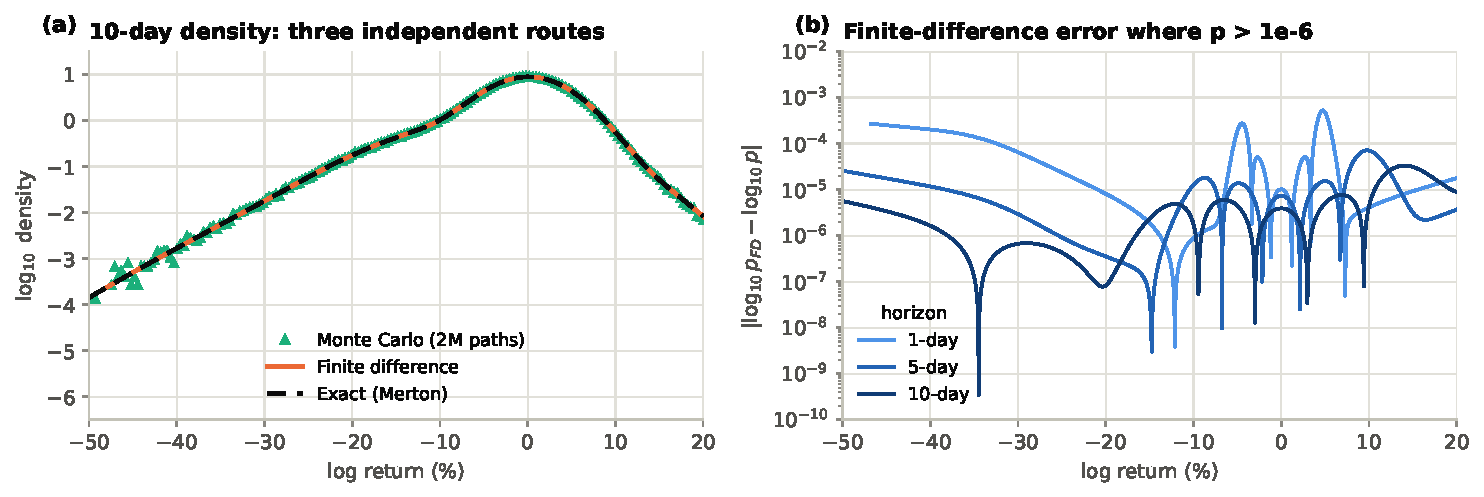
\includegraphics[width=\linewidth]{stage2_reference/fig02_fd_mc_validation.pdf}
  \caption{Stage 2 reference solvers against the Merton closed form: FD and Monte Carlo densities and their
    errors. FD is used as the 1-D baseline from here on.}
  \label{fig:ref1d}
\end{figure}

\subsection{The 1-D PINN}
With 48 Gauss--Hermite nodes for the jump integral the 1-D PINN reaches relative errors below 1\% for every
VaR and ES at 95--99.9\% and all three horizons (maximum 0.61\%). ES$_{99}$ errors are 0.30\%, 0.42\% and
0.16\% at 1, 5 and 10 days (\cref{fig:pinn1d}). The tail is learned as well as the bulk: the left-tail
mean absolute error in $\log p$ is 0.015 at 1 day. Training takes 8.6 minutes and a full density query
1.4\,ms. In one dimension the FD solver is both more accurate (errors of order $10^{-6}$) and faster
(0.34\,s), so the 1-D study validates the method rather than motivating it.

\begin{figure}[t]
  \centering
  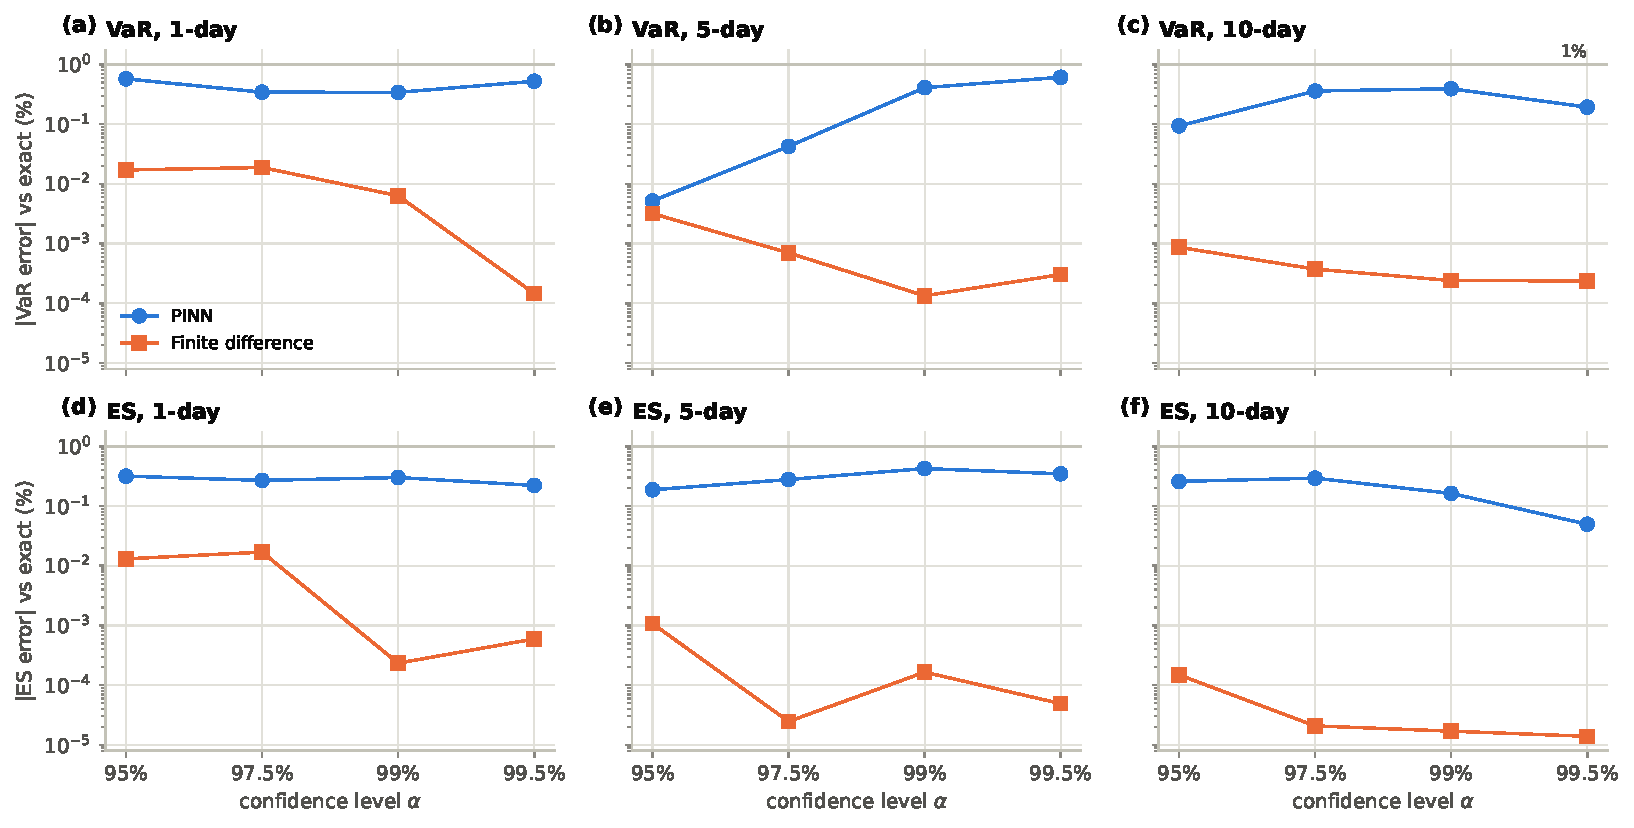
\includegraphics[width=\linewidth]{stage2_pinn1d/fig05_var_es_error.pdf}
  \caption{1-D PINN: relative VaR and ES error against the closed form, by confidence level and horizon.}
  \label{fig:pinn1d}
\end{figure}

\subsection{Ablations}
\Cref{tab:ablation} removes one design choice at a time, with three seeds each. Three components are
essential. The \emph{log-form residual} (writing the PIDE for $\log p$ rather than $p$) is the largest
single factor: without it, 10-day ES errors exceed 50\%. The \emph{resolution of the jump quadrature} sets
the short-horizon accuracy: at 1 day the error falls from 12--15\% with 8 nodes to about 2\% with 24 and
0.2--0.3\% with 48. The \emph{normalisation penalty} is needed at short horizons (2.2\% without it). Tail-adaptive
collocation, by contrast, gave no measurable gain and was dropped from Stage 4 onwards.

\begin{table}[t]
  \centering
  \caption{1-D ablations: ES$_{99}$ relative error, range over three seeds
    (\texttt{results/stage2\_ablation\_seeds.csv}).}
  \label{tab:ablation}
  \begin{tabular}{lcc}
    \toprule
    Variant & 1 day & 10 days \\
    \midrule
    Baseline (log residual, 48 nodes, normalisation) & 0.18--0.30\% & 0.06--0.16\% \\
    Linear residual (on $p$)                         & 0.9--22\%    & 57--152\% \\
    8 quadrature nodes                               & 12--15\%     & 0.2--0.8\% \\
    24 quadrature nodes                              & 1.7--2.1\%   & 0.01--0.18\% \\
    No normalisation penalty                         & 2.1--2.2\%   & 0.07--0.14\% \\
    No tail-adaptive collocation                     & 0.06--0.36\% & 0.04--0.05\% \\
    \bottomrule
  \end{tabular}
\end{table}

% ------------------------------------------------------------------------------------------------
\section{Multi-asset ground truth}
\label{sec:res-ref2d}

For $d = 2$ a Douglas ADI finite-difference scheme with an FFT line kernel for the common jump was built as
an independent check of the closed form. It converges at second order ($L^1$ error 0.027 on a $101^2$ grid,
0.0068 on $201^2$) and reproduces portfolio ES within 0.012\% (Monte Carlo: 0.3\%). Its cost, however, grows
from 0.3\,s for the 1-D grid to 55\,s for a $401^2$ grid, and a $d$-dimensional grid grows as $n^d$
(\cref{fig:fdcost}). Beyond three assets grid methods are not usable, and Monte Carlo and the closed form are
the only references in the scaling study.

\begin{figure}[t]
  \centering
  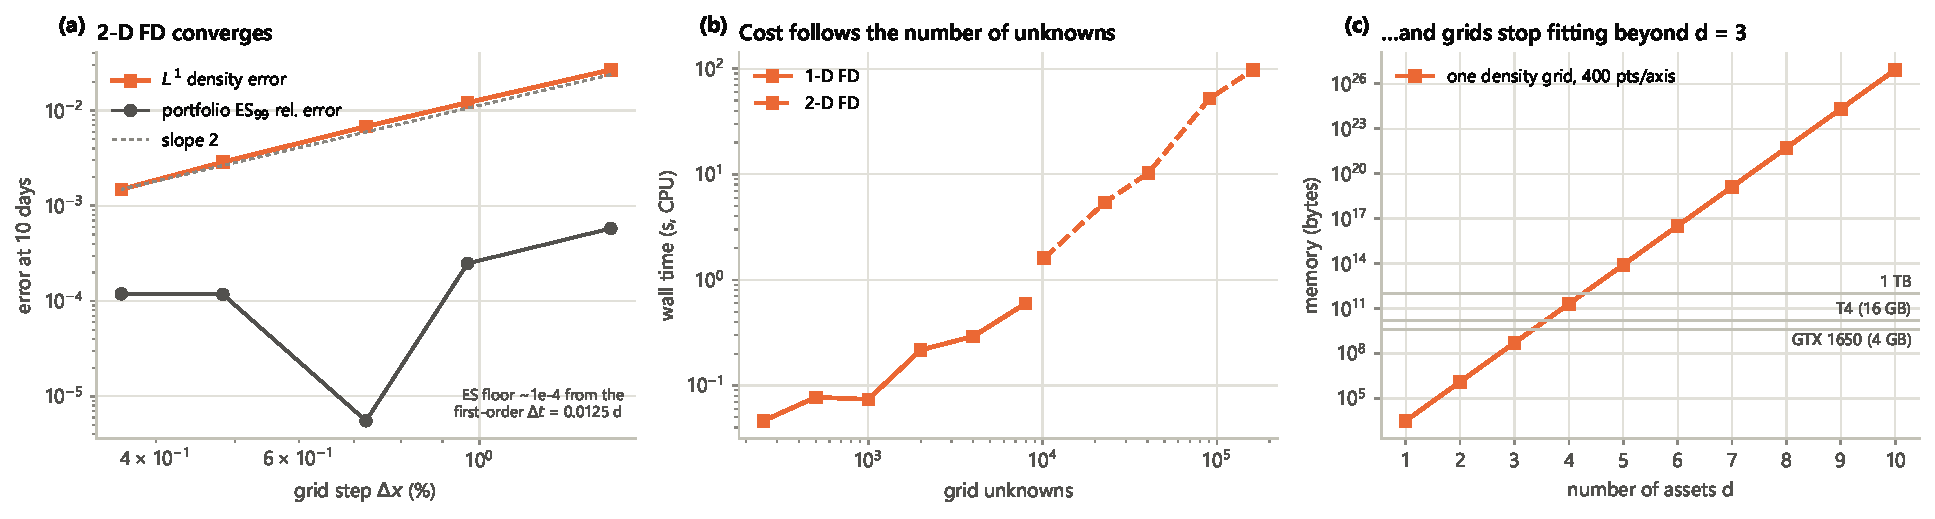
\includegraphics[width=\linewidth]{stage3_multiasset_reference/fig02_fd_cost.pdf}
  \caption{Cost and accuracy of the 2-D FD reference against grid size; the 1-D solver for comparison.}
  \label{fig:fdcost}
\end{figure}

% ------------------------------------------------------------------------------------------------
\section{Scaling with dimension (RQ1, RQ4)}
\label{sec:res-scaling}

The $d$-dimensional PINN uses the same network (width 128, depth 4) and 20{,}000 steps for every $d$. The
Laplacian is computed exactly for $d \le 2$ and with Hutchinson's estimator for $d \ge 5$.
\Cref{tab:scaling} and \cref{fig:scaling} report the result.

\begin{table}[t]
  \centering
  \caption{Scaling with dimension: median ES$_{99}$ error over 20 portfolios, the IS floor and Monte Carlo
    at the same budget, the tail log-density error at 1 day, and training time on a T4
    (\texttt{results/stage4\_summary.csv}).}
  \label{tab:scaling}
  \begin{tabular}{llcccccc}
    \toprule
    $d$ & trace & \multicolumn{2}{c}{PINN} & \multicolumn{2}{c}{MC (same $N$)} & tail MAE & train \\
        &       & 1 day & 10 days & 1 day & 10 days & $\log p$ & (min) \\
    \midrule
    1  & exact      & 1.4\% & 0.05\% & 1.1\% & 0.22\% & 0.03 & 9.4 \\
    2  & exact      & 0.7\% & 1.0\%  & 1.4\% & 1.6\%  & 0.02 & 10.5 \\
    5  & Hutchinson & 1.1\% & 0.6\%  & 0.2\% & 0.4\%  & 0.05 & 12.8 \\
    5  & exact      & 0.09\% & 1.4\% & 0.2\% & 0.4\%  & 0.14 & 13.6 \\
    10 & Hutchinson & 5.2\% & 62\%   & 0.6\% & 0.8\%  & 0.20 & 13.3 \\
    \bottomrule
  \end{tabular}
\end{table}

Up to five assets the PINN stays at or below about 1\% ES$_{99}$ error, within the range of Monte Carlo at
the same budget, with training time almost flat in $d$ (9.4 to 13.6 minutes). Hutchinson's estimator is
as accurate as the exact trace at $d = 5$, so the cost of the Laplacian is not the limit.

At $d = 10$ the method breaks: the PDE loss stalls at 0.76 (0.14 at $d = 5$), and the learned density is
too wide along the jump direction $\beta$ while remaining correct across it. The error grows with horizon,
from 5\% at 1 day to 62\% at 10 days. Following the fallback in the research plan, $d = 10$ is reported as
the breakdown point of this architecture and training budget, and the later stages use $d \le 5$.

\begin{figure}[t]
  \centering
  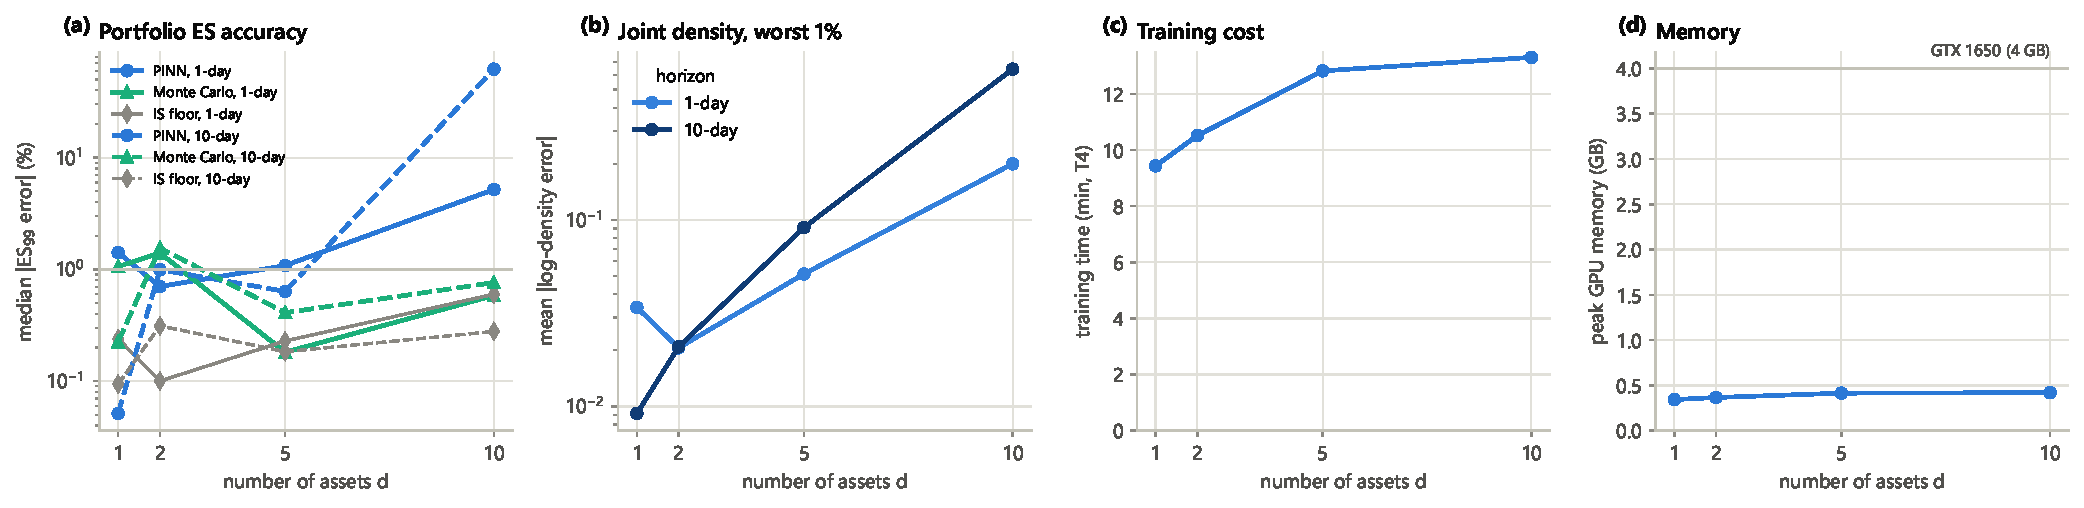
\includegraphics[width=\linewidth]{stage4_summary/fig01_scaling.pdf}
  \caption{ES$_{99}$ error against dimension for the PINN, Monte Carlo at the same budget and the IS floor.}
  \label{fig:scaling}
\end{figure}

% ------------------------------------------------------------------------------------------------
\section{Amortised real-time risk (RQ5)}
\label{sec:res-amortised}

The amortised PINN takes the model parameters $\theta = (s, \lambda, \mu_J)$ as additional inputs: a
volatility multiplier $s \in [0.6, 1.6]$, a jump intensity $\lambda \in [1, 15]$/yr and a mean jump size
$\mu_J \in [-0.10, -0.02]$. One network trained once (18 minutes at $d = 2$, 22 minutes at $d = 5$) then
answers risk queries for any $\theta$ in this box without retraining.

\paragraph{Accuracy over $\theta$.} Over the $(s, \lambda)$ evaluation grid the median ES$_{99}$ error at
1/5/10 days is 1.3/0.8/0.7\% at $d = 2$, against 1.8/0.9/0.8\% for Monte Carlo at the same $N$. At $d = 5$
it is 1.3/1.8/3.4\% against 1.4/0.9/0.7\%: the amortised model matches Monte Carlo at 1 day but degrades with
horizon, and its worst cells reach 10\% (10 days, $s = 0.6$, $\lambda = 15$) and 7\% (high $s$, low
$\lambda$) (\cref{fig:amortised}).

\paragraph{Sensitivities.} Because the density is a differentiable function of $w$ and $\theta$, Euler
risk contributions $\partial \ES / \partial w_i$ and what-if curves come from one model. Euler contributions
agree with finite differences of the exact ES to within about 5\%. ES($\lambda$) follows the exact curve;
ES($s$) has a bias of up to 1.3 percentage points at intermediate $s$.

\paragraph{Latency.} At matched error Monte Carlo is faster: 0.9--1.6\,ms per query against 4--18\,ms
for PINN importance sampling, so the break-even analysis finds no query count at which the PINN pays back
its training cost. This is expected for Merton, where exact simulation costs no more than drawing from the
proposal. The value of the amortised PINN under this model is therefore a smooth, differentiable surrogate in
$\theta$ (for sensitivities and scenario analysis), not raw speed. A speed advantage requires a model whose
simulation is expensive, which is outside the scope of this work.

\begin{figure}[t]
  \centering
  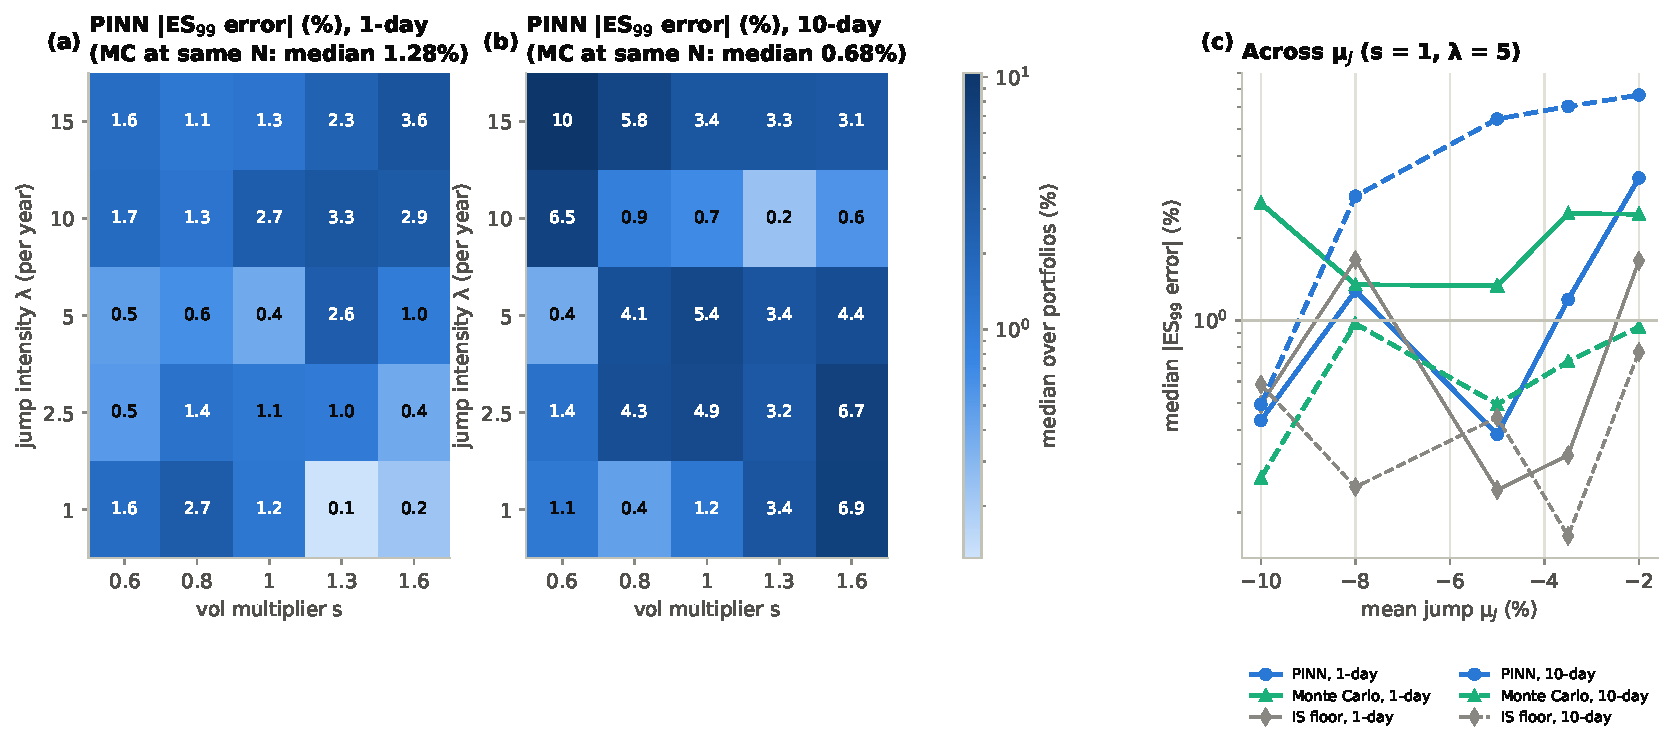
\includegraphics[width=\linewidth]{stage5_amortised_d5/fig02_accuracy_theta.pdf}
  \caption{Amortised PINN at $d = 5$: ES$_{99}$ error over the $(s, \lambda)$ grid at each horizon.}
  \label{fig:amortised}
\end{figure}

% ------------------------------------------------------------------------------------------------
\section{Real-data backtests (RQ2)}
\label{sec:res-real}

\paragraph{Setup.} Two five-asset baskets are used: NIFTY (Reliance, HDFC Bank, Infosys, ICICI Bank, TCS)
and S\&P sector ETFs (XLK, XLF, XLE, XLV, XLI). Daily data run from January 2006 to October 2026; models are
developed on data up to December 2017 and tested from January 2018 (2,176 and 2,217 test days, including the
COVID crash). The filtered Merton model has a daily volatility scale from EWMA filtering and jump parameters
fitted by maximum likelihood, with MAP shrinkage of the rolling $(\lambda, \mu_J)$ towards the development fit.
The PINN is trained once per market over the box of parameters seen in development, then queried every day.
It is compared with Gaussian, historical simulation (HS), filtered HS (FHS), GARCH-$t$, EVT, DCC and an
unfiltered Merton model, on a linear basket and on a non-linear book (basket plus a short 3\%-out-of-the-money
one-month put).

\paragraph{Calibration findings.} Real-data jumps are small and frequent: $\lambda \approx 20$/yr with
$\sigma_J = 2.4\%$ for NIFTY and $\lambda \approx 100$/yr with $\sigma_J = 0.9\%$ for S\&P. They act as a
variance mixture rather than as rare crashes.

\paragraph{The PINN reproduces its model.} Against the exact filtered-Merton density on the same importance
draws, the PINN's daily ES error has median (maximum) 2.8\% (7\%) on NIFTY and 0.2\% (1.7\%) on S\&P at 99\%,
and breach counts are identical (\cref{tab:backtest}). One failure required a fix. On 2022-06-16 a single
proposal draw about 100 standard deviations out received all the importance weight, because the PINN, never
trained there, decays more slowly than the proposal. Draws more than six radii from the nearest collocation
component are now discarded. This removes at most $2\times10^{-16}$ of exact mass and at most 0.9\% of draws,
and keeps the effective sample size above 54\%. The cause is examined in \cref{sec:res-failure}.

\begin{table}[t]
  \centering
  \caption{Linear-basket backtests at 99\%, January 2018 -- October 2026, sorted by the FZ0 joint
    VaR--ES score (lower is better). $p_{\mathrm{uc}}$: Kupiec; $p_{\mathrm{cc}}$: Christoffersen;
    $p_{\mathrm{DM}}$: Diebold--Mariano test of FZ0 against the PINN
    (\texttt{results/stage6\_realdata\_*/backtest.csv}).}
  \label{tab:backtest}
  \small
  \begin{tabular}{llrrrrrr}
    \toprule
    Market & Model & Breaches & Rate & $p_{\mathrm{uc}}$ & $p_{\mathrm{cc}}$ & FZ0 & $p_{\mathrm{DM}}$ \\
    \midrule
    \multirow{9}{*}{NIFTY}
      & DCC             & 28 & 1.29\% & 0.20 & 0.29 & $-3.301$ & 0.004 \\
      & FHS             & 19 & 0.87\% & 0.54 & 0.31 & $-3.278$ & 0.14 \\
      & GARCH-$t$       & 31 & 1.42\% & 0.06 & 0.13 & $-3.205$ & 0.38 \\
      & EVT             & 26 & 1.19\% & 0.38 & 0.41 & $-3.201$ & 0.36 \\
      & \textbf{PINN}   & 15 & 0.69\% & 0.12 & 0.27 & $-3.156$ & -- \\
      & Merton (exact)  & 15 & 0.69\% & 0.12 & 0.27 & $-3.134$ & -- \\
      & HS              & 26 & 1.19\% & 0.38 & 0.008 & $-3.016$ & 0.05 \\
      & Gaussian        & 38 & 1.75\% & 0.002 & $<$0.001 & $-2.881$ & 0.12 \\
      & Merton (unfilt.) & 25 & 1.15\% & 0.50 & $<$0.001 & $-2.672$ & 0.10 \\
    \midrule
    \multirow{9}{*}{S\&P}
      & EVT             & 20 & 0.90\% & 0.64 & 0.04 & $-3.353$ & 0.04 \\
      & GARCH-$t$       & 32 & 1.44\% & 0.05 & 0.03 & $-3.322$ & 0.06 \\
      & DCC             & 33 & 1.49\% & 0.03 & $<$0.001 & $-3.294$ & 0.07 \\
      & FHS             & 20 & 0.90\% & 0.64 & 0.04 & $-3.244$ & 0.14 \\
      & \textbf{PINN}   & 27 & 1.22\% & 0.32 & 0.009 & $-3.046$ & -- \\
      & Merton (exact)  & 27 & 1.22\% & 0.32 & $<$0.001 & $-3.044$ & -- \\
      & HS              & 30 & 1.35\% & 0.11 & $<$0.001 & $-2.731$ & 0.004 \\
      & Merton (unfilt.) & 36 & 1.62\% & 0.007 & $<$0.001 & $-2.533$ & 0.02 \\
      & Gaussian        & 59 & 2.66\% & $<$0.001 & $<$0.001 & $-2.297$ & 0.01 \\
    \bottomrule
  \end{tabular}
\end{table}

\paragraph{Backtest results.} At 99\% the filtered Merton model, and hence the PINN, passes the Kupiec test
on both markets and the Christoffersen test on NIFTY. On S\&P, breaches cluster for almost every model and
conditional coverage is rejected nearly everywhere. At 97.5\% the model is conservative (breach rate 1.75\%
on NIFTY, 1.80\% on S\&P) and Kupiec rejects on both markets. On the joint FZ0 score the PINN beats the
Gaussian, HS and unfiltered Merton models (significantly on S\&P), but volatility-driven models with
fat-tailed innovations do better: on NIFTY, FHS passes every test and DCC is significantly better than the PINN;
on S\&P, EVT, GARCH-$t$ and DCC are better, significantly so at 97.5\%. Results on the non-linear book rank the
models in the same order. The PINN costs 8.7\,ms per day on a T4, against 13\,ms for the exact density.

The conclusion for RQ2 is that the PINN is a faithful and cheap surrogate of the jump-diffusion model, and its
backtest performance is that of the model: competitive with classical methods, better than Gaussian and
unfiltered alternatives, but not better than the best GARCH/EVT-type forecasters on these baskets.

\begin{figure}[t]
  \centering
  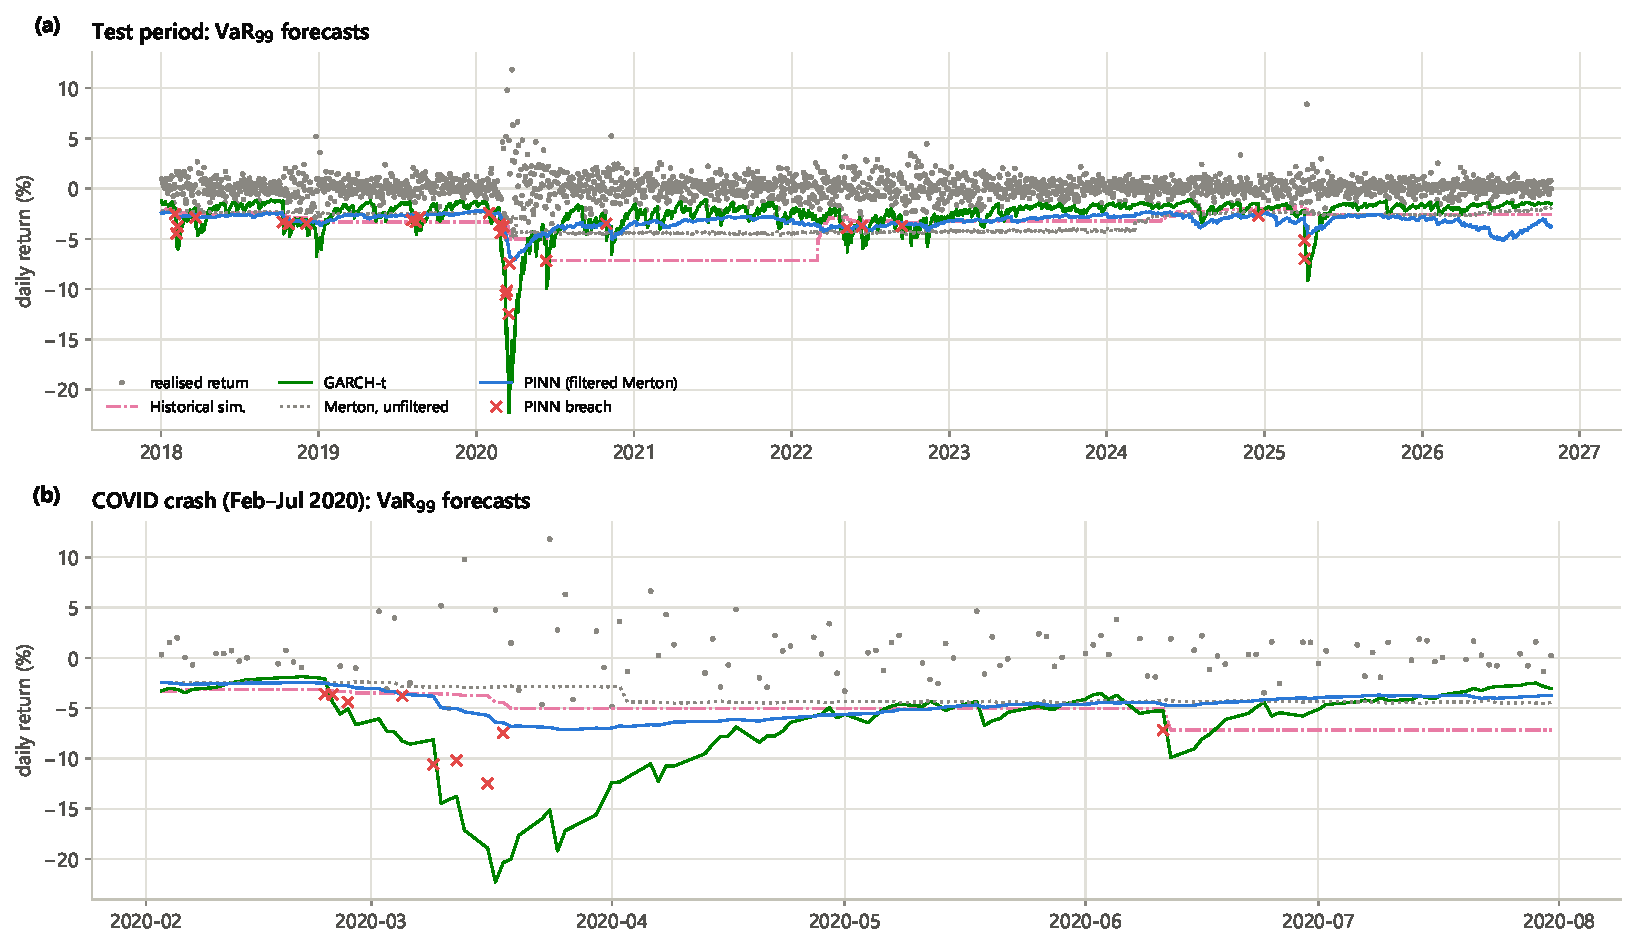
\includegraphics[width=\linewidth]{stage6_realdata_sp/fig03_var_paths.pdf}
  \caption{S\&P basket: daily 99\% VaR forecasts of the PINN and benchmarks against realised returns,
    2018--2026.}
  \label{fig:varpaths}
\end{figure}

% ------------------------------------------------------------------------------------------------
\section{Physics versus data, and failure cases (RQ3)}
\label{sec:res-ablation}

\subsection{Physics-informed versus data-only}
To isolate the contribution of the physics, the PINN was compared with a \emph{data-only} network that is
identical in architecture, optimiser, learning-rate schedule, number of steps and normaliser estimator, but
is trained by maximum likelihood on $N$ exact samples instead of the PIDE. The samples are spread over 16
times in $[t_0, T]$, 20\% are held out for early stopping, and $N$ ranges from $10^3$ to $10^6$ with three
seeds each. Monte Carlo on the same samples is the third method, and all models are weighted on the same
importance draws, so differences between them are model differences.

\begin{table}[t]
  \centering
  \caption{Physics versus data: median ES$_{99}$ error over 20 portfolios (data-only and Monte Carlo:
    median over three seeds). The PINN uses no samples
    (\texttt{results/stage7\_physics\_vs\_data\_d*/metrics.json}).}
  \label{tab:physdata}
  \begin{tabular}{llccc@{\hspace{2em}}ccc}
    \toprule
    & & \multicolumn{3}{c}{$d = 2$} & \multicolumn{3}{c}{$d = 5$} \\
    Method & $N$ & 1 day & 5 days & 10 days & 1 day & 5 days & 10 days \\
    \midrule
    PINN (physics)   & 0       & 1.3\% & 0.9\% & 0.08\% & 1.8\% & 2.2\% & 0.8\% \\
    \midrule
    \multirow{4}{*}{Data-only NN}
      & $10^3$ & 21\%  & 4.7\% & 1.7\% & 44\% & 28\% & 64\% \\
      & $10^4$ & 13\%  & 2.1\% & 3.8\% & 13\% & 5.7\% & 9.2\% \\
      & $10^5$ & 5.0\% & 0.8\% & 2.5\% & 3.3\% & 1.8\% & 3.2\% \\
      & $10^6$ & 1.3\% & 0.4\% & 0.18\% & 2.8\% & 0.8\% & 0.8\% \\
    \midrule
    \multirow{4}{*}{MC, same samples}
      & $10^3$ & 75\% & 16\% & 34\% & 68\% & 32\% & 23\% \\
      & $10^4$ & 23\% & 7.1\% & 9.7\% & 11\% & 8.1\% & 6.0\% \\
      & $10^5$ & 7.8\% & 5.2\% & 1.6\% & 11\% & 3.2\% & 1.5\% \\
      & $10^6$ & 0.8\% & 1.2\% & 1.1\% & 2.1\% & 0.7\% & 1.6\% \\
    \bottomrule
  \end{tabular}
\end{table}

\Cref{tab:physdata} and \cref{fig:physdata} give the answer to RQ3. The PINN, which sees no samples, is worth
roughly $10^5$ to $10^6$ exact samples. The data-only network reaches the PINN's 5-day error at about
$6.6\times10^4$ samples in both dimensions; at 1 and 10 days it does not reach it before $10^6$. With the sample
sizes available in practice (a few thousand daily observations), data-only errors are 5--60\%. The data-only
network is itself better than Monte Carlo on the same samples at small $N$, since it smooths across times, but
both need of order $10^6$ samples to reach the accuracy the physics provides for free.

This comparison should be read with one caveat. When the model is known, one can always simulate, so the
PINN's advantage is not that samples are unavailable. Its advantage is that one training run gives a smooth,
normalised and differentiable density at every time in $[t_0, T]$, which can be amortised over parameters
(\cref{sec:res-amortised}) and differentiated for risk contributions, at no sampling cost per query.

\begin{figure}[t]
  \centering
  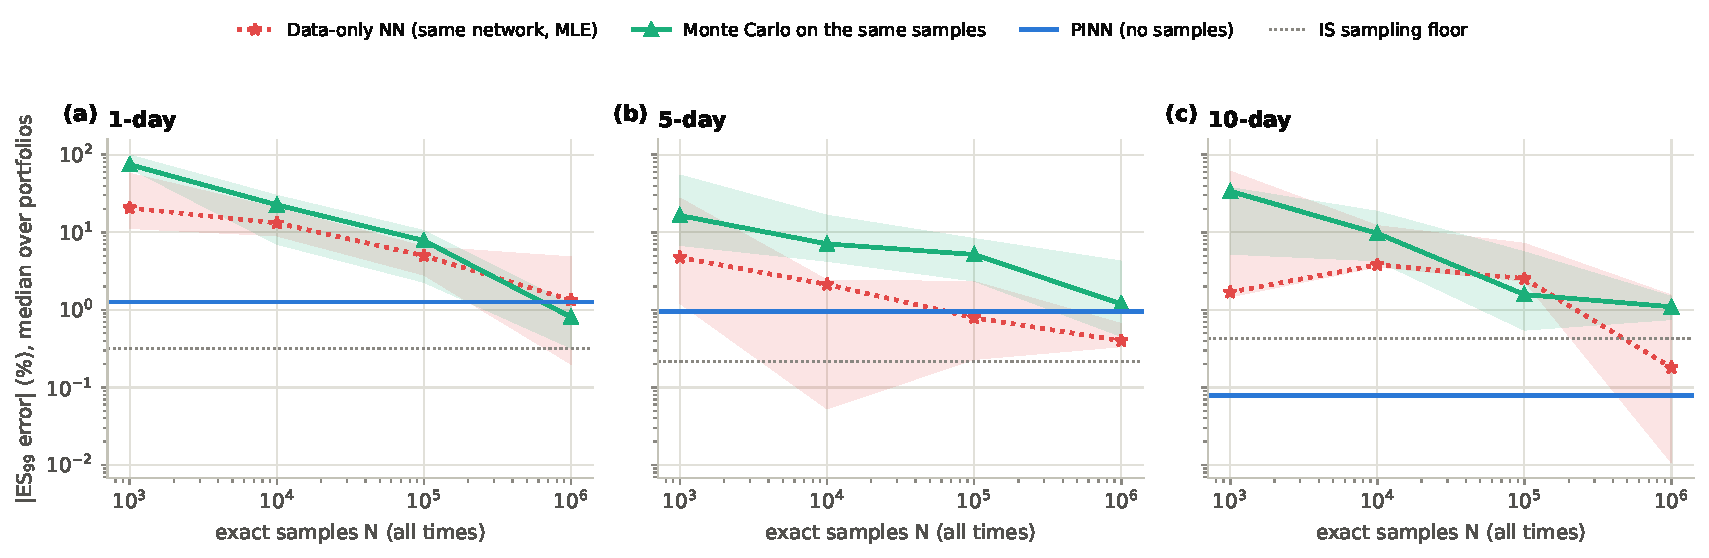
\includegraphics[width=\linewidth]{stage7_physics_vs_data_d2/fig02_es_vs_samples.pdf}
  \caption{$d = 2$: ES$_{99}$ error against the number of exact samples for the data-only network (red) and
    Monte Carlo on the same samples (green); the PINN uses none (blue line). Bands: range over seeds.}
  \label{fig:physdata}
\end{figure}

\subsection{Failure cases}
\label{sec:res-failure}
Three controlled changes to the $d = 2$ setup test the method's assumptions, and two failures from earlier
stages are collected with them (\cref{tab:failure}, \cref{fig:failure}).

\begin{table}[t]
  \centering
  \caption{Failure cases: median ES$_{99}$ error over portfolios
    (\texttt{results/stage7\_final/failure\_cases.csv}).}
  \label{tab:failure}
  \begin{tabular}{lccc}
    \toprule
    Case & 1 day & 5 days & 10 days \\
    \midrule
    $d = 2$, Stage 4 reference                    & 0.70\% & 0.69\% & 0.99\% \\
    $\lambda = 50$/yr, proposal $k \le 3$ jumps    & 0.59\% & 0.74\% & 0.78\% \\
    $\lambda = 50$/yr, proposal $k \le 10$ jumps   & 0.29\% & 0.07\% & 0.12\% \\
    $t_0 = 0.05$ day                               & \textbf{5.2\%} & 0.94\% & 0.25\% \\
    $d = 5$ amortised, worst $\theta$ (Stage 5)    & 3.6\% & 4.7\% & \textbf{10\%} \\
    $d = 10$ (Stage 4)                             & \textbf{5.2\%} & \textbf{44\%} & \textbf{62\%} \\
    \bottomrule
  \end{tabular}
\end{table}

\paragraph{High jump intensity.} At $\lambda = 50$/yr the default proposal covers at most three jumps, while
the probability of more jumps reaches 14\% at 10 days. Contrary to the expectation, the PINN does not break:
the error stays below 1\%, because the residual loss still trains the network where the proposal is thin.
Widening the proposal to ten jumps reduces the error by a factor of five to ten. The jump coverage of the
proposal is therefore a tuning choice, not a hard limit.

\paragraph{Short start time.} Starting at $t_0 = 0.05$ day instead of 0.5 day makes the initial density ten
times sharper. This is a genuine failure at short horizons: the 1-day ES$_{99}$ error is 5.2\%, the 1-day VaR$_{99}$
error 21\%, and the tail log-density error 0.13 (0.02 for the reference). The error decays as the density
widens, to 0.25\% at 10 days. Short horizons need either a $t_0$ close to the first horizon of interest or a
time rescaling that keeps the initial density resolvable.

\paragraph{Dimension and parameter range.} The $d = 10$ breakdown (\cref{sec:res-scaling}) and the worst corner
of the $d = 5$ amortised box (\cref{sec:res-amortised}) are the largest errors in the study. Both grow with
horizon, so they come from error accumulating along the time direction rather than from the initial condition.

\paragraph{Far-tail extrapolation.} \Cref{fig:failure}(b) traces $\log p - \log q$ along rays from the centre.
For the exact density it falls to between $-50$ and $-230$ at 150 whitened units; for the PINN it turns positive
beyond about 20 units and keeps rising. Outside the trained region the network decays more slowly than the
heavy-tailed proposal, so a single far-out draw can carry all the importance weight. This is the mechanism behind
the S\&P blow-up in \cref{sec:res-real}, and it justifies the trust region used there. The PINN's density is
reliable only within the region covered by its collocation points.

\begin{figure}[t]
  \centering
  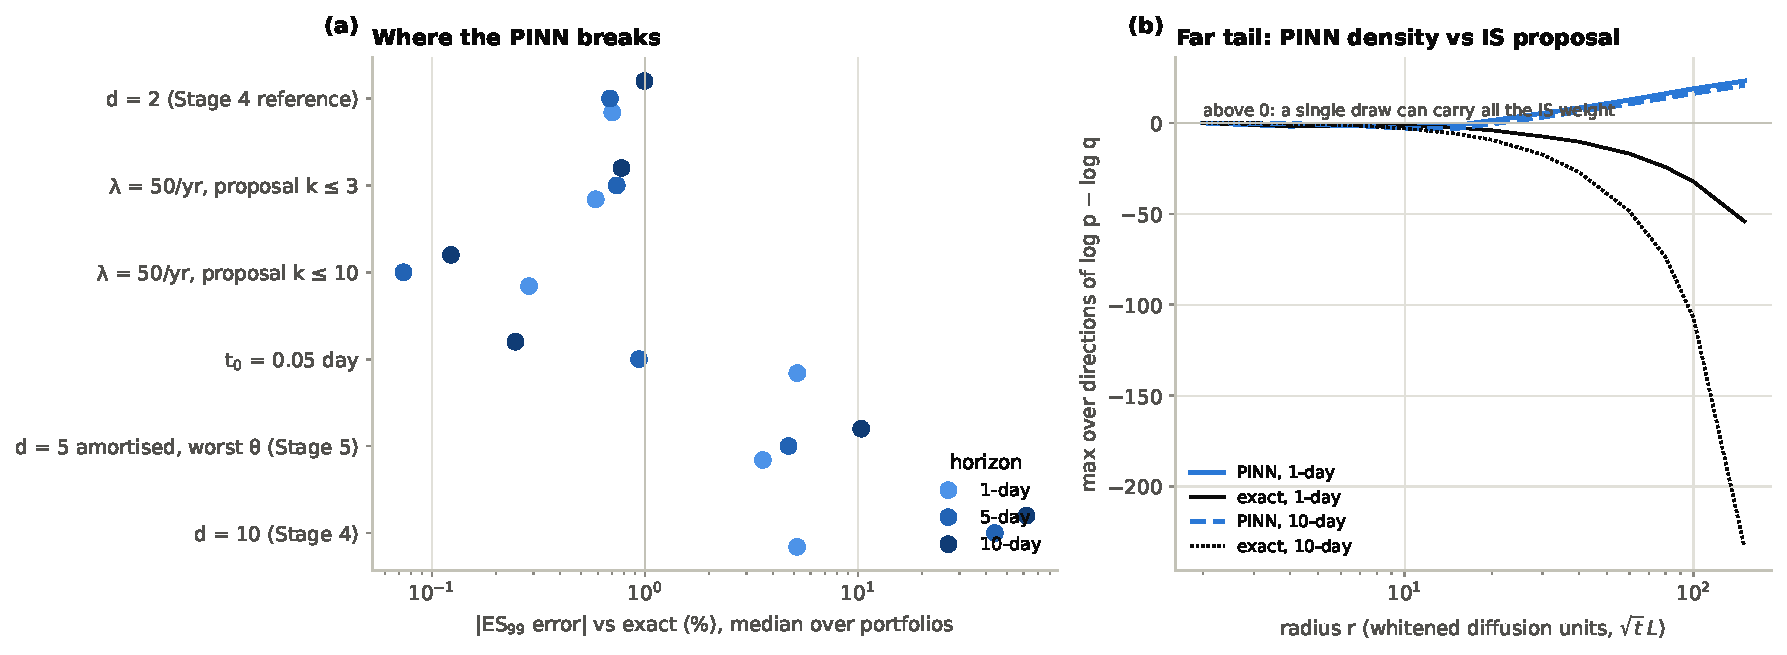
\includegraphics[width=\linewidth]{stage7_final/fig02_failure_cases.pdf}
  \caption{(a) ES$_{99}$ error by failure case and horizon; the vertical line marks 1\%. (b) Far-tail probe:
    the maximum over 2,000 directions of $\log p - \log q$ for the PINN and the exact density.}
  \label{fig:failure}
\end{figure}

% ------------------------------------------------------------------------------------------------
\section{Summary and answers to the research questions}
\label{sec:res-summary}

\Cref{fig:scorecard} places the PINN's ES$_{99}$ error next to its baseline in every stage.

\begin{figure}[t]
  \centering
  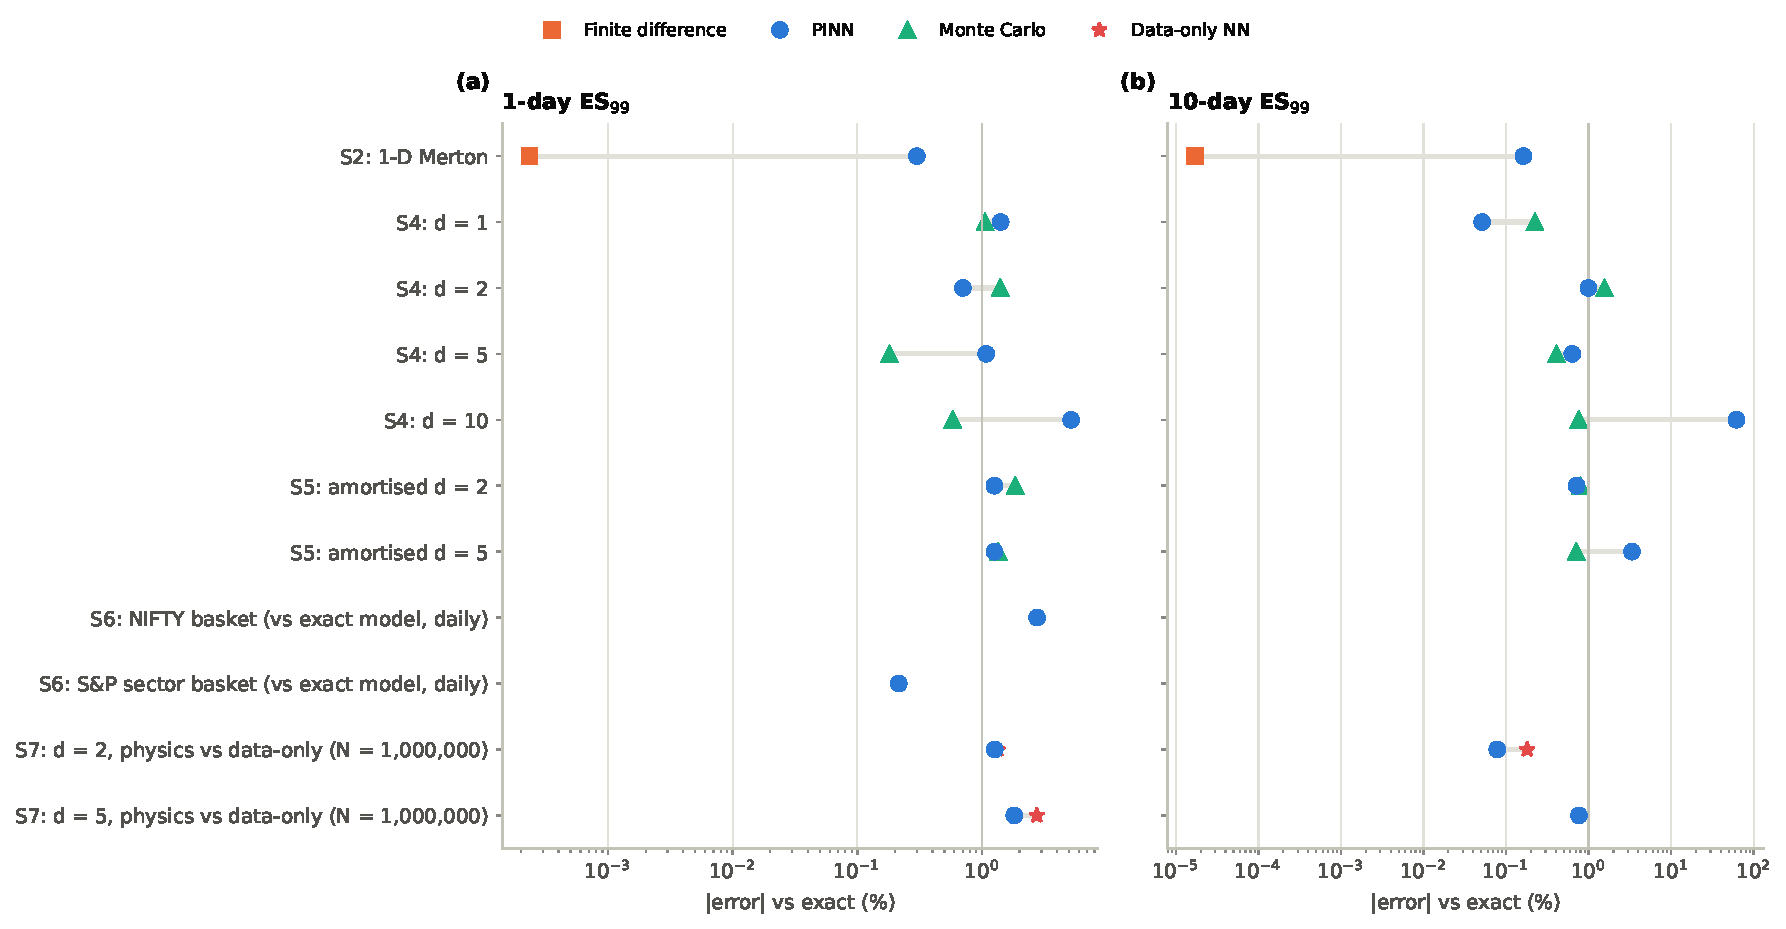
\includegraphics[width=\linewidth]{stage7_final/fig01_scorecard.pdf}
  \caption{Scorecard over Stages 2--7: PINN ES$_{99}$ error (blue) against the baseline of each stage
    (FD, Monte Carlo at the same budget, or the data-only network), at 1 and 10 days.}
  \label{fig:scorecard}
\end{figure}

\begin{description}
  \item[RQ1 (bulk versus tail).] With the log-form residual the tail is learned as accurately as the bulk:
    tail log-density errors are 0.015--0.05 for $d \le 5$, and ES errors are at or below 1\%. The tail fails
    first at the limits: at $d = 10$ (tail error 0.20), for a very sharp initial density, and beyond the
    collocation region, where the density is not constrained at all.
  \item[RQ2 (calibration on real data).] The PINN reproduces the filtered Merton model to within 0.2--2.8\%
    in daily ES with identical breaches. The model passes unconditional coverage at 99\% on both markets but is
    conservative at 97.5\%, and on the FZ0 score it is beaten by FHS, DCC, GARCH-$t$ and EVT while beating
    Gaussian, HS and unfiltered Merton.
  \item[RQ3 (physics versus data).] The physics replaces roughly $10^5$--$10^6$ exact samples. At realistic
    sample sizes a data-only network of the same design is 5--60\% off.
  \item[RQ4 (scaling).] One architecture and training budget works up to $d = 5$ at about 1\% error, with
    training time nearly flat in $d$, where grid methods are already impractical beyond $d = 3$. It breaks at
    $d = 10$.
  \item[RQ5 (latency).] A single amortised network answers queries over the whole parameter box in 4--18\,ms,
    with sensitivities by differentiation. For the Merton model Monte Carlo is faster at matched error, so there
    is no break-even; a speed advantage requires models whose simulation is expensive.
\end{description}

\paragraph{Limitations.} All synthetic results use a model with a common jump factor, which keeps the jump
integral one-dimensional; idiosyncratic jumps would need a $d$-dimensional integral. The multi-asset method was
not made to work at $d = 10$. The real-data comparison tests the jump-diffusion model as much as the PINN, and
the volatility filter, not the PINN, determines most of the backtest result.
